\subsection{Context and motivation of PhD}

\begin{frame}{Introduction}{Context and motivation of PhD}
	\begin{block}{\textbf{Context and motivation}}
		The railway system is responsible for 1.3\% of entire European energy consumption, \cite{iea-uic2016}. 
		The debate on energy efficiency in railways is a well-discussed topic due to its impact on the global energy consumption.
		
		The energy efficiency analysis and management requires a detailed mapping of the energy consumption/generation in the railway system. 
		This detailed mapping of the energy flows should include, not only the rolling stock level but also the traction substations and the auxiliary services.
		The knowledge of all the load curves permits load prevision, peak shaving and energy cost optimization for the entirely of the railway system.
		
	\end{block}
\end{frame}
%%%%%%%%%%%%%%%%%%%%%%%%%%%%%%%%%%%%%%%%%%%%%%%%%%%%%%%%%%%%%%%%%%%%%%%%%%%%%%%%%%%%%

\subsection{Shift2Rail Framework}
\begin{frame}{Introduction}{Shift2Rail Framework}
\begin{block}{\textbf{Shift2Rail Framework - Main Goal}}
	\begin{itemize}
		\setlength\itemsep{-0.5em}
		\item 1. Cutting the life-cycle cost of railway transport by, at least, 50\%;
		\item 2. Doubling the railway capacity;
		\item 3. Increasing the reliability and punctuality by 50\%, at least.
	\end{itemize}
	
\end{block}
\end{frame}
%%%%%%%%%%%%%%%%%%%%%%%%%%%%%%%%%%%%%%%%%%%%%%%%%%%%%%%%%%%%%%%%%%%%%%%%%%%%%%%%%%%%%

\begin{frame}{Introduction}{Shift2Rail Framework}
\begin{block}{\textbf{Shift2Rail Framework - Time Targets}}
	Complementary, the time target goals are the establishment of a framework, by 2020, for a European multimodal transport system for the passenger rail, freight and for the urban mobility. By 2030 is expected to triple the length of the existing high-speed passenger rail network, 30\% of the road freight over 300 km should shift to rail or waterborne transport and achieve a CO2-free city logistics in major urban centers. By 2050, the medium-distance passenger transport should go by rail and high-speed rail, with the connection of all core network airports to the high-speed railway network. On the freight is expected to have all seaports connected to the rail freight transport system and on the urban mobility, the "conventionally-fueled" cars will not have place in cities by 2050, \cite{shift2rail2015}.
	
\end{block}
\end{frame}
%%%%%%%%%%%%%%%%%%%%%%%%%%%%%%%%%%%%%%%%%%%%%%%%%%%%%%%%%%%%%%%%%%%%%%%%%%%%%%%%%%%%%

\begin{frame}{Introduction}{Shift2Rail Framework}
\begin{block}{\textbf{Shift2Rail Framework - Innovation Programmes}}
The \ac{S2R} carries five innovation programmes, as presented in figure \ref{fig:ips}. Framed on the S2R \ac{IP3} with the focus on the ”Cost efficient and reliable infrastructure”, it is proposed the development of a \ac{SMD} that achieves a detailed monitoring and supervision of various energy flows on the premises of embracing the entire \ac{RTS}.
\end{block}


\begin{figure}[h!]
	\centering
	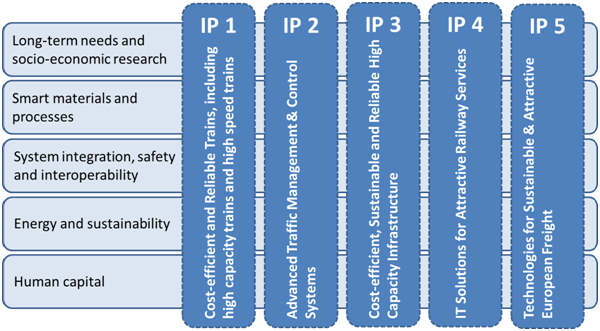
\includegraphics[width=0.60\textwidth,keepaspectratio]{figures/1.Intro/IPs}
	\caption{Shif2Rail Innovation Programs. }
	\label{fig:ips}
\end{figure}


\end{frame}
%%%%%%%%%%%%%%%%%%%%%%%%%%%%%%%%%%%%%%%%%%%%%%%%%%%%%%%%%%%%%%%%%%%%%%%%%%%%%%%%%%%%%

\subsection{Main Goal}
\begin{frame}{Introduction}{}
\begin{block}{\textbf{Main Goal}}
The purpose of any energy management strategy is to build the dynamics of every loads and generators of the power system. 
This should be performed based on an extensive knowledge of every energy flows. 
This way, the \ac{SMD} is required to propose and validate a standard metering architecture that involves the coordination of every measurement performed either in on-board and in ground. 
In advance, energy data analysis should be provided based on relevant stored data. 

\end{block}
\end{frame}
%%%%%%%%%%%%%%%%%%%%%%%%%%%%%%%%%%%%%%%%%%%%%%%%%%%%%%%%%%%%%%%%%%%%%%%%%%%%%%%%%%%%%